	The business layer, organised into different modules, is built through an object-oriented paradigm and it is used by the \gls{rest} API to retrieve or update state and behaviour. For instance, the content, routing and personalisation packages are built according to the grammatical rules that \gls{cawiml} defines in its \gls{xsd} schema. These three packages are widely used across the survey stages and following sections provide a high-level view of the different modules that are involved in each of the client stages of design, collection and management analytics.

	\subsubsection{The design stage}

	The Validation and Parser packages are crucial at the questionnaire design stage as these carry out the validation, correctness and translation of \gls{xml} constructs into artefacts that are ready for data gathering. Particularly, the parser package reads data from valid \gls{xml} specifications to produce objects according to the content, routing and personalisation modules. It uses an event-driven approach that handles a variety of small to large questionnaire specifications appropriately. The event-driven style when compared to the popular \gls{dom} parsing, uses significantly less resources since there is no need to create a tree of objects in memory representing the \gls{xml} file under process.
	%Additionally, when the parsing task is completed, routines such as the creation of Variables according to the questions (see Section \ref{sec:design:factoryPattern}) or the binding of piping features (e.g. text-fills and carry-forward) to questions are performed. Specifically, the late bindings are carried out at the end since \gls{xml} instances according to \gls{ssm} have forward references to objects that are still not created since the parser reads \gls{xml} files from top to bottom (e.g. XML FILE EXAMPLE FROM SSM).

	\subsubsection{The collection stage}

	The collection stage uses the state-transition model expressed in a \gls{cawiml} instance to conduct interviews. The class diagram from Figure \ref{fig:design:collection} represents an overview of the most important classes involved. A state model consisting of states and transitions, holds variables that represent the questions from a section and their responses. Additionally, it keeps references to pipes that together with the pseudo states, use the \gls{rpn} formalism to execute logical and arithmetical expressions. The routing class, contains a list of state models and an entry point to mark the state model execution entry point. It also holds the set of place holder variables (e.g. Field class) that are shared across state models.

	\begin{figure}[h]
	\centering
	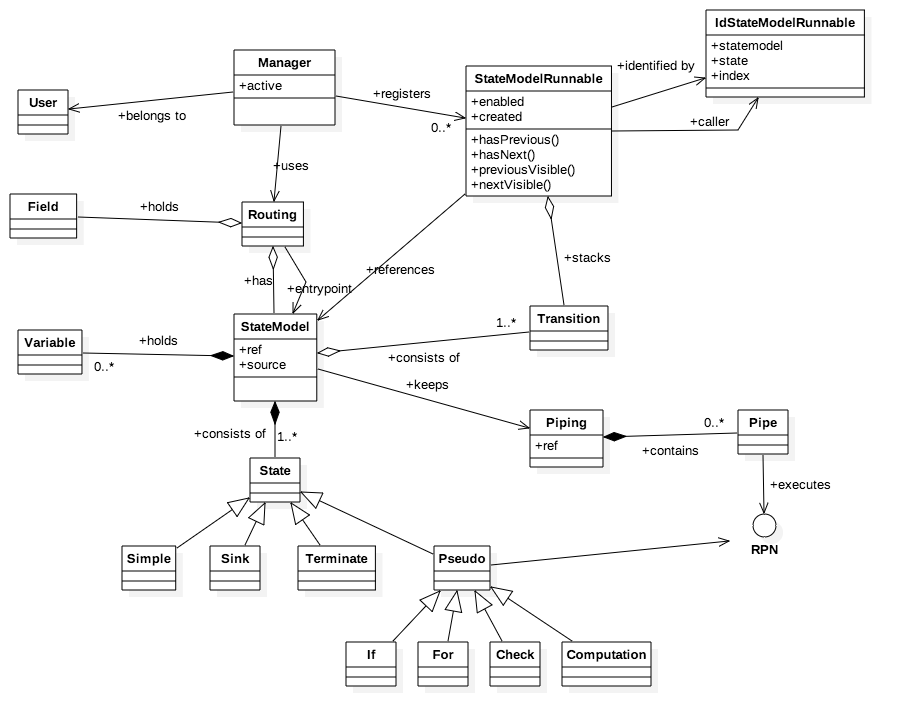
\includegraphics[max size={\textwidth}{\textheight}]{design/img/collectionManager.png}
	\caption{Class diagram for the Collection Manager}
	\label{fig:design:collection}
	\end{figure}

	Each interviewee (e.g. User class) has a Manager object that registers the set of state models defined in a state-transition and controls which state model is active at any time. The state modelRunnable class, adds behaviour to a state model by including methods such as hasPrevious(), hasNext(), previousVisible() and nextVisible() that permit navigating backward and forward through an interview. It contains interesting properties like \emph{created}, that registers the date and time in which the state model was generated, and \emph{enabled}, that determines whether or not the state model variables should be considered when data is exported or visualised on client interfaces. The instances of this class are typically identified by a state model and state (e.g. IdStatemodelRunnable) but also may contain an index if the state model is part of a loop. For instance, the inner state model from Figure \ref{fig:design:stateTransition}, that represents the questionnaire from Figure \ref{fig:background:survey}, can have up to eight different state modelRunnable instances identified by outer and 'c1' for the state model and the state respectively. Also an index that varies from 01 to 08 according to the set of response codes from Q2 or Q3 is set to identify each state model copy uniquely.

	\subsubsection{The management, analysis and reporting stages}

	The management stage, aimed at monitoring the data gathered in real time, fetches questionnaire objects by conducting multiple queries against the persistence layer. For instance, status objects are sent to the client in order to inform the percentage of completion of a questionnaire or to determine accurately the current question in an interview session.

	The analysis stage incorporate aggregate queries to study the data collection for questionnaires for each type of question. For instance, an attractive feature that calculates the degree of positivity for open string questions, automatically separates sentences into one of six categories (e.g. strong positive, positive, weak positive, weak negative, negative or strong negative) proposed by Haque and Tamjid \cite{art:haque14} by using the word scores from SentiWordNet \cite{proc:esuli06}. %This module, firstly separates negative and positive terms of a sentence through a tokenisation process \cite{web:apache16}, secondly calculates the weighted average score for each term according to SentiWordNet \cite{proc:esuli06} and thirdly calculates the degree of the sentence by taking the highest absolute negative or positive score. This value obtained ranges from -1 to 1 and the sentence falls into one of the six categories (e.g. strong positive, positive, weak positive, weak negative, negative or strong negative) proposed by Haque and Tamjid \cite{art:haque14}.

	The reporting stage offers mechanisms to export survey data and meta data into \gls{csv} format currently. This process uses a variation of the Topological Sort algorithm proposed by Kahn \cite{art:kahn62} to retrieve the order of the questions as they are defined in the routing of the \gls{cawiml} specification and presents the survey meta data first followed by the data for each interviewee on each successive line.

	